


\paragraph{STM32 Nucleo-F722ZE}\label{sec:stm32-nucleo-f722ze}\mbox{}\\

\textbf{\hyperlink{lf-nn-01}{/LF03/}} \\

\begin{wrapfigure}{r}{0.4\textwidth} % Increase the width of the figure environment
	\vspace{-10pt}
	\hspace{20pt}
	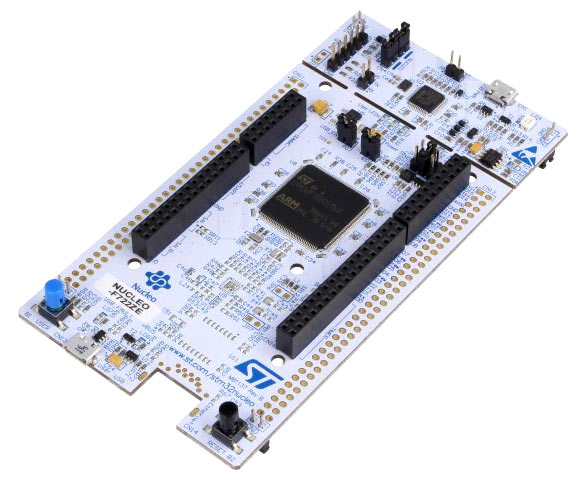
\includegraphics[width=0.25\textwidth]{images/05_technische_spezifikation/nn/nucleo_f722ze.jpg}
	\caption{STM32 Nucleo-F722ZE Board}
	\label{fig:nucleo-f722ze}
\end{wrapfigure}


Das in \textbf{Abbildung \ref{fig:nucleo-f722ze}} gezeigte STM32 Nucleo-F722ZE Board integriert einen Microcontroller und wird in erster Linie für den Betrieb des neuronalen Netzes benötigt. Auf diesem Board soll jedoch das gesamte Projekt umgesetzt werden. Nachdem noch keine Erfahrungen mit dem Ressourcenverbrauch von neuronalen Netzen auf Microcontrollern gesammelt wurden, wurde dieses Board ausgewählt, da es über mehr Ressourcen verfügt als die Nucleo-F7401RE Boards. Dadurch soll sicher gestellt werden, dass bei der Integration aller Komponenten nicht zu Ressourcenknappheiten, insbesondere beim RAM, kommt.

Es verfügt im Vergleich zum STM32 Nucleo-F401RE Board über mehr SRAM (256 Kbytes vs. 96 Kbytes) und über eine leistungsstärkere CPU (Cortex M7 CPU mit 462 DMIPS/2.14 DMIPS vs. Cortex M4 CPU mit 105 DMIPS/1.25 DMIPS) \cite{stm32F7-board}. 

Das Board wird mit einer Versorgungsspannung von 5V betrieben. 